\documentclass[final,6p,times,twocolumn]{elsarticle}
\setlength{\parindent}{20pt} % esp. al inicio de un parrafo
\usepackage{url}
\usepackage{doi}
\usepackage{listings}
\usepackage{xcolor}
\usepackage{caption}
\usepackage{subcaption}
\makeatletter

\renewenvironment{abstract}{\global\setbox\absbox=\vbox\bgroup
  \hsize=\textwidth\def\baselinestretch{1}%
  \noindent\unskip\textbf{Resumen}  % <--- Edit as necessary
 \par\medskip\noindent\unskip\ignorespaces}
 {\egroup}

\def\keyword{%
  \def\sep{\unskip, }%
 \def\MSC{\@ifnextchar[{\@MSC}{\@MSC[2000]}}
  \def\@MSC[##1]{\par\leavevmode\hbox {\it ##1~MSC:\space}}%
  \def\PACS{\par\leavevmode\hbox {\it PACS:\space}}%
  \def\JEL{\par\leavevmode\hbox {\it JEL:\space}}%
  \global\setbox\keybox=\vbox\bgroup\hsize=\textwidth
  \normalsize\normalfont\def\baselinestretch{1}
  \parskip\z@
  \noindent\textit{Palabras clave: }  % <--- Edit as necessary
  \raggedright                         % Keywords are not justified.
  \ignorespaces}

\usepackage[spanish]{babel}

\def\ps@pprintTitle{%
     \let\@oddhead\@empty
     \let\@evenhead\@empty
     \def\@oddfoot{\footnotesize\itshape
        \ifx\@journal\@empty   % <--- Edit as necessary
       \else\@journal\fi\hfill\today}%
     \let\@evenfoot\@oddfoot}

%% The graphicx package provides the includegraphics command.
\usepackage{graphicx}
%% The amssymb package provides various useful mathematical symbols
\usepackage{amssymb}
%% The amsthm package provides extended theorem environments
\usepackage{amsthm}

\usepackage{amsmath}

%% The lineno packages adds line numbers. Start line numbering with
%% \begin{linenumbers}, end it with \end{linenumbers}. Or switch it on
%% for the whole article with \linenumbers after \end{frontmatter}.
\usepackage{lineno}


%% natbib.sty is loaded by default. However, natbib options can be
%% provided with \biboptions{...} command. Following options are
%% valid:

%%   round  -  round parentheses are used (default)
%%   square -  square brackets are used   [option]
%%   curly  -  curly braces are used      {option}
%%   angle  -  angle brackets are used    <option>
%%   semicolon  -  multiple citations separated by semi-colon
%%   colon  - same as semicolon, an earlier confusion
%%   comma  -  separated by comma
%%   numbers-  selects numerical citations
%%   super  -  numerical citations as superscripts
%%   sort   -  sorts multiple citations according to order in ref. list
%%   sort&compress   -  like sort, but also compresses numerical citations
%%   compress - compresses without sorting
%%
%% \biboptions{comma,round}

% \biboptions{}

%\journal{Journal Name}

\hypersetup{
    colorlinks=true,
    linkcolor=blue,
    filecolor=blue,      
    urlcolor=blue,
}
\renewcommand{\lstlistingname}{C\'odigo}
\definecolor{codegreen}{rgb}{0,0.6,0}
\definecolor{codegray}{rgb}{0.5,0.5,0.5}
\definecolor{codepurple}{rgb}{0.58,0,0.82}
\definecolor{backcolour}{rgb}{0.95,0.95,0.92}
\lstdefinestyle{mystyle}{
    backgroundcolor=\color{backcolour},   
    commentstyle=\color{codegreen},
    keywordstyle=\color{magenta},
    numberstyle=\tiny\color{codegray},
    stringstyle=\color{codepurple},
    basicstyle=\ttfamily\footnotesize,
    breakatwhitespace=false,         
    breaklines=true,                 
    keepspaces=true,                 
    numbers=left,                    
    numbersep=5pt,                  
    showspaces=false,                
    showstringspaces=false,
    showtabs=false,                  
    tabsize=2
}
\lstset{style=mystyle}

\begin{document}

\begin{frontmatter}

%% Title, authors and addresses

\title{Modelado de nanoindentaci\'on de una pel\'icula delgada de oro}

%% use the tnoteref command within \title for footnotes;
%% use the tnotetext command for the associated footnote;
%% use the fnref command within \author or \address for footnotes;
%% use the fntext command for the associated footnote;
%% use the corref command within \author for corresponding author footnotes;
%% use the cortext command for the associated footnote;
%% use the ead command for the email address,
%% and the form \ead[url] for the home page:
%%
%% \title{Title\tnoteref{label1}}
%% \tnotetext[label1]{}
%% \author{Name\corref{cor1}\fnref{label2}}
%% \ead{email address}
%% \ead[url]{home page}
%% \fntext[label2]{}
%% \cortext[cor1]{}
%% \address{Address\fnref{label3}}
%% \fntext[label3]{}


%% use optional labels to link authors explicitly to addresses:
%% \author[label1,label2]{<author name>}
%% \address[label1]{<address>}
%% \address[label2]{<address>}

\author{Jorge A. Torres Quintanilla}

\address{Posgrado en Maestr\'ia en Ciencias de la Ingenier\'ia con Orientaci\'on en Nanotecnolog\'ia.}

\address{Facultad de Ingenier\'ia Mec\'anica y El\'ectrica.}

\address{Universidad Aut\'onoma de Nuevo Le\'on.}

\begin{abstract}
    Debido su alta relaci\'on \'area/volumen, los materiales a escala nanom\'etrica presentan propiedades f\'isicoqu\'imicas que los diferenc\'ian del material en bulto. Es por esto que se han desarrollado modelos matem\'aticos que describan con mayor precisi\'on el comportamiento de las interacciones de los materiales a estas escalas. Los estudios de nanoindentaci\'on hacen uso de estos modelos y de la rama de la mec\'anica de contacto para deducir las propiedades mec\'anicas y adhesivas (como dureza, ductilidad, fuerza de adhesi\'on), de un sinf\'in de materiales. En este art\'iculo se realiza la simulaci\'on computacional de un nanoindentador de diamante entrando en contacto con una pel\'icula delgada de oro. Se calculan las profundidades de indentaci\'on y se comparan con datos experimentales con el fin de elucidar en la veracidad de dichos modelos. Los resultados muestran diferencias significativas entre los datos reales y los te\'oricos, pero hay similitudes en la forma del comportamiento, lo cual puede indicar que hay otros fen\'omenos que no se est\'an tomando en cuenta en la simulaci\'on.
\end{abstract}

\begin{keyword}
Mec\'anica de contacto \sep nanoindentaci\'on \sep adhesi\'on \sep simulaci\'on
\end{keyword}

\end{frontmatter}

\section{Introducci\'on}
La mec\'anica de contacto es un \'area de la tribolog\'ia que estudia la deformaci\'on de s\'olidos que se tocan entre s\'i en uno o más puntos. Se hace una distinci\'on entre los esfuerzos que act\'uan en un objeto de manera perpendicular (normal) y los que son causados por fricci\'on, que tienen una direcci\'on tangencial entre superficies. El estudio de estos esfuerzos y deformaciones es especialmente \'util para determinar las propiedades mec\'anicas y adhesivas que presentan los materiales, como la dureza, m\'odulo el\'astico y punto de fractura.

En la rama de la nanotecnolog\'ia, los materiales presentan una alta relaci\'on \'area/volumen comparada al material en bulto, lo cual altera sus propiedades mec\'anicas y adhesivas. Esto implica que deben proponerse modelos matem\'aticos que definan con mayor precisi\'on el comportamiento de la materia a tales escalas. Los estudios de nanoindentaci\'on son pruebas muy comunes en este \'ambito de la ciencia, y se utilizan para determinar un rango de propiedades que presentan los nanomateriales. Estas pruebas consisten en la aplicaci\'on de una fuerza al material cuyas propiedades se desean saber por medio de una punta muy fina con geometr\'ia y propiedades mec\'anicas conocidas, usualmente de diamante o un material de alta dureza. Esto se hace con el prop\'osito de causar una indentaci\'on en el material estudiado, cuya geometr\'ia est\'a directamente relacionada con sus propiedades mec\'anicas y de adhesi\'on.

En el presente se propone una simulaci\'on de los dos modelos m\'as com\'unmente utilizados en estudios de nanoindentaci\'on, con un enfoque espec\'ifico en las propiedades de una pel\'icula delgada de oro. Los resultados se comparan con datos reales obtenidos de pruebas de nanoindentaci\'on realizadas por Beake y Smith \cite{BEAKE2002} bajo condiciones similares.

\section{Antecedentes}
Experimentos como los realizados por Beake y Smith \cite{BEAKE2002} y Dietker \textit{et al.} \cite{DIETIKER2008} ya han utilizado la t\'ecnica de nanoindentaci\'on para medir las propiedades mec\'anicas de diversos materiales, incluyendo pel\'iculas delgadas de oro. Los anteriores se basan en el modelo de contacto el\'astico descrito por Hertz \cite{HERTZ} y en la t\'ecnica desarrollada por Oliver y Pharr \cite{OLIVER1992}, con la cual determinan el m\'odulo el\'astico y la dureza de diversos materiales por medio de la gr\'afica carga-profundidad. Un ejemplo de este tipo de gr\'afica se puede observar en la figura \ref{fig1}.

\begin{figure}
    \centering
    \includegraphics[scale=0.24]{Images/Gold P-h graph.png}
    \caption{Gr\'afica carga-profundidad de una pel\'icula de oro \cite{BEAKE2002}.}
    \label{fig1}
\end{figure}

\section{Trabajos Relacionados}
En su trabajo, Kelchner \textit{et al.} \cite{KELCHNER1998} realizan la simulaci\'on de una prueba de nanoindentaci\'on de una pel\'icula delgada de oro con dimensiones de $24\times21\times16$ nm y un indentador de geometr\'ia esf\'erica con un radio de $8$ nm. Hacen uso de un modelo de din\'amica molecular paralela para simular el comportamiento de $470,000$ \'atomos al entrar en contacto con el indentador, as\'i como de las ecuaciones descritas en el modelo Hertziano. Sus resultados son muy prometedores, ya que no solamente encuentran que el comportamiento simulado se acerca en buena medida al real, sino que pueden determinar puntos de dislocaci\'on en la estructura cristalina del oro.

\section{Modelo Propuesto}\label{mod}
En el presente se hace uso de los dos modelos m\'as com\'unmente utilizados en el \'ambito de mec\'anica de contacto. El primero de ellos es el descrito por Hertz \cite{HERTZ}, en el cual no se toman en cuenta las propiedades adhesivas de los materiales, por lo que la profundidad de indentaci\'on est\'a determinada \'unicamente por la fuerza aplicada $F$, el m\'odulo el\'astico reducido de ambos materiales en contacto $E^*$, y la dimensi\'on caracter\'istica del indentador $R$, como se puede apreciar en la ecuaci\'on \ref{eq1}.

\begin{equation}\label{eq1}
    d_{HERTZ} = \left( \frac{9F^2}{16E{^*}{^2}R} \right)^\frac{1}{3}
\end{equation}

El m\'odulo el\'astico reducido $E^*$ es una funci\'on de los m\'odulos el\'asticos $(E_1, E_2)$, y de las relaciones de Poisson $(\nu_1, \nu_2)$, de ambos materiales, como se expresa en la ecuaci\'on \ref{eq2}.

\begin{equation}\label{eq2}
    \frac{1}{E^*}=\frac{1-\nu_1^2}{E_1} + \frac{1-\nu_2^2}{E_2}
\end{equation}

El segundo modelo es el descrito por Johnson, Kendall y Roberts (JKR) \cite{JKR}, en el cual toman en cuenta la energ\'ia de adhesi\'on existente entre ambas superficies, por lo que el \'area de contacto resultante es mayor que la descrita por el modelo Hertziano, y cuya profundidad de indentaci\'on depende ahora del trabajo de adhesi\'on ejercido entre ambos materiales $\Delta\gamma$ y de las presiones ejercidas por la fuerza aplicada $(p_0, p^\prime_0)$, como se observa en la ecuaci\'on \ref{eq3}.

\begin{equation}\label{eq3}
    d_{JKR}=\frac{\pi a_{JKR}}{2E^*}\left( p_0 + 2p^\prime_0 \right)
\end{equation}

Las presiones $p_0$ y $p^\prime_0$ est\'an determinadas por la ecuaci\'on \ref{eq4}, donde los t\'erminos $a_{JKR}$ y $\Delta\gamma$ son el \'area de contacto descrita por el modelo JKR y el trabajo de adhesi\'on ejercido entre ambas superficies, los cuales se encuentran expresados en las ecuaciones \ref{eq5} y \ref{eq6}, respectivamente. $\gamma_1$ y $\gamma_2$ son las energ\'ias de adhesi\'on de cada uno de los materiales en contacto, mientras que $\gamma_{12}$ es el t\'ermino de interacci\'on.

\begin{equation}\label{eq4}
    p_0 = \frac{2a_{JKR} E^*}{\pi R} ; p^\prime_0 = -\left( \frac{2\Delta\gamma E^*}{\pi a_{JKR}} \right)^\frac{1}{2}
\end{equation}

\begin{multline}\label{eq5}
a_{JKR} = \Bigg\{ \frac{3R}{4E^*} \Bigg[ \Bigg. F + 3\Delta\gamma\pi{R} \\
+ \sqrt{6\Delta\gamma\pi{R}{F} + (3\Delta\gamma\pi{R})^2} \Bigg. \Bigg] \Bigg\}^\frac{1}{3}
\end{multline}

\begin{equation}\label{eq6}
    \Delta\gamma = \gamma_1 + \gamma_2 - \gamma_{12}
\end{equation}

Para los modelos matem\'aticos presentados, se propone la simulaci\'on de un nanoindentador con una punta de diamante tipo Berkovich, de geometr\'ia esf\'erica con un radio $R=200$ nm. El m\'odulo el\'astico reducido se obtiene de datos experimentales realzados por Dietiker \textit{et al.} \cite{DIETIKER2008}, y se toma como $E^* = 85$ GPa. El trabajo de adhesi\'on entre el diamante y el oro se toma como $\Delta\gamma = 300$ $mJ/m^2$, dados los datos obtenidos experimentalmente por Gane \textit{et al.} \cite{GANE1974}. Por \'ultimo, la fuerza aplicada $F$ se aumenta gradualmente en un rango de 0 - 50 mN, y se calculan las profundidades de indentaci\'on descritas por las ecuaciones de ambos modelos. La teor\'ia apunta a una diferencia significativa entre ambos modelos en las profundidades de indentaci\'on a cargas muy bajas, mientras que esta diferencia ir\'ia disminuyendo conforme se aumenta la carga aplicada.

\section{Implementaci\'on}
La simulaci\'on se implementa con el software de desarrollo Python v3.10.1 \cite{PY}, mientras que el c\'odigo completo se puede encontrar en el repositorio en GitHub de Torres \cite{jorge1}.

En el c\'odigo \ref{codigo1} se toman datos reales de una curva carga-profundidad de experimentos realizados en pel\'iculas de oro por Beake y Smith \cite{BEAKE2002}. As\'imismo, se introducen los par\'ametros de geometr\'ia, m\'odulo el\'astico y trabajo de adhesi\'on descritos en la secci\'on \ref{mod}.

\begin{lstlisting}[caption=Datos Experimentales y Par\'ametros de Operaci\'on, label=codigo1, language=Python]
datos = pd.read_csv('DatosReales.txt', delimiter = ' ')

F = (datos.Carga)*(10**-3) #N
d_r = datos.Deformacion
E = 85*(10**9) #Pa
R = 200*(10**-9) #m
g = 300*(10**-3) #J/m2
\end{lstlisting}

Las l\'ineas del c\'odigo \ref{codigo2} introducen las listas donde se guardan los valores calculados de profundidades de indentaci\'on para ambos modelos, as\'i como las diferencias de profundidad entre los datos experimentales y los calculados.

\begin{lstlisting}[caption=Listas de Profundidades de Indentaci\'on y Diferencias, label=codigo2, language=Python]
hertz_list = []
jkr_list = []
diffa = []
diffb = abs(d_r - hertz_list)
diffc = abs(d_r - jkr_list)
\end{lstlisting}

Las funciones \texttt{a()}, \texttt{d\_hertz} y \texttt{d\_jkr} del c\'odigo \ref{codigo3} definen las ecuaciones para calcular el \'area de contacto seg\'un el modelo JKR, $a_{JKR}$, la profundidad de indentaci\'on seg\'un el modelo Hertziano, $d_{HERTZ}$, y la profundidad de indentaci\'on seg\'un el modelo JKR, $d_{JKR}$, respectivamente.

\begin{lstlisting}[caption=Funciones de Ecuaciones de los Modelos, label=codigo3, language=Python]
def a(F):
    return (((3*R)/(4*E))*(F + 3*g*pi*R + np.sqrt((6*g*pi*R*F) + (3*g*pi*R)**2)))**(1/3)

def d_hertz(F):
    return (((9*(F**2))/(16*(E**2)*R)) **(1/3))*(10**9)

def d_jkr(F, a, p1, p2):
    return (((pi*a)/(2*E))*(p1 + 2*p2)) *(10**9)
\end{lstlisting}

En el c\'odigo \ref{codigo4} se comienza a introducir la fuerza debido al indentador, y se calculan el \'area de contacto, $a_{JKR}$, los componentes de presi\'on, $p_0$ y $p^\prime_0$, as\'i como las profundidades de indentaci\'on, $d_{HERTZ}$ y $d_{JKR}$. Para cada dato de fuerza aplicada se calcula la diferencia entre las profundidades Hertzianas y de JKR y se agregan a la lista.

\begin{lstlisting}[caption=Implementaci\'on de Modelos Matem\'aticos, label=codigo4, language=Python]
for f in F:
    A = a(f)
    p1 = (2*A*E)/(pi*R)
    p2 = -1 * np.sqrt((2*g*E)/(pi*A))
    hertz = d_hertz(f)
    jkr = d_jkr(f, A, p1, p2)
    hertz_list.append(hertz)
    jkr_list.append(jkr)
    diffa.append(abs(jkr - hertz))
\end{lstlisting}

\section{Resultados}
En la figura \ref{fig2} se observa una comparaci\'on entre las gr\'aficas carga-profundidad de los datos experimentales y los calculados con el modelo Hertziano (figura \ref{fig2a}) y los calculados con el modelo JKR (figura \ref{fig2b}).

La figura \ref{fig3} muestra los errores absolutos en profundidades de indentaci\'on entre ambos modelos (figura \ref{fig3a}), entre los datos experimentales y el modelo Hertziano (figura \ref{fig3b}), y entre los datos experimentales y el modelo JKR (figura \ref{fig3c}).

\begin{figure}
\centering
    \begin{subfigure}[t]{0.49\textwidth}
         \centering
         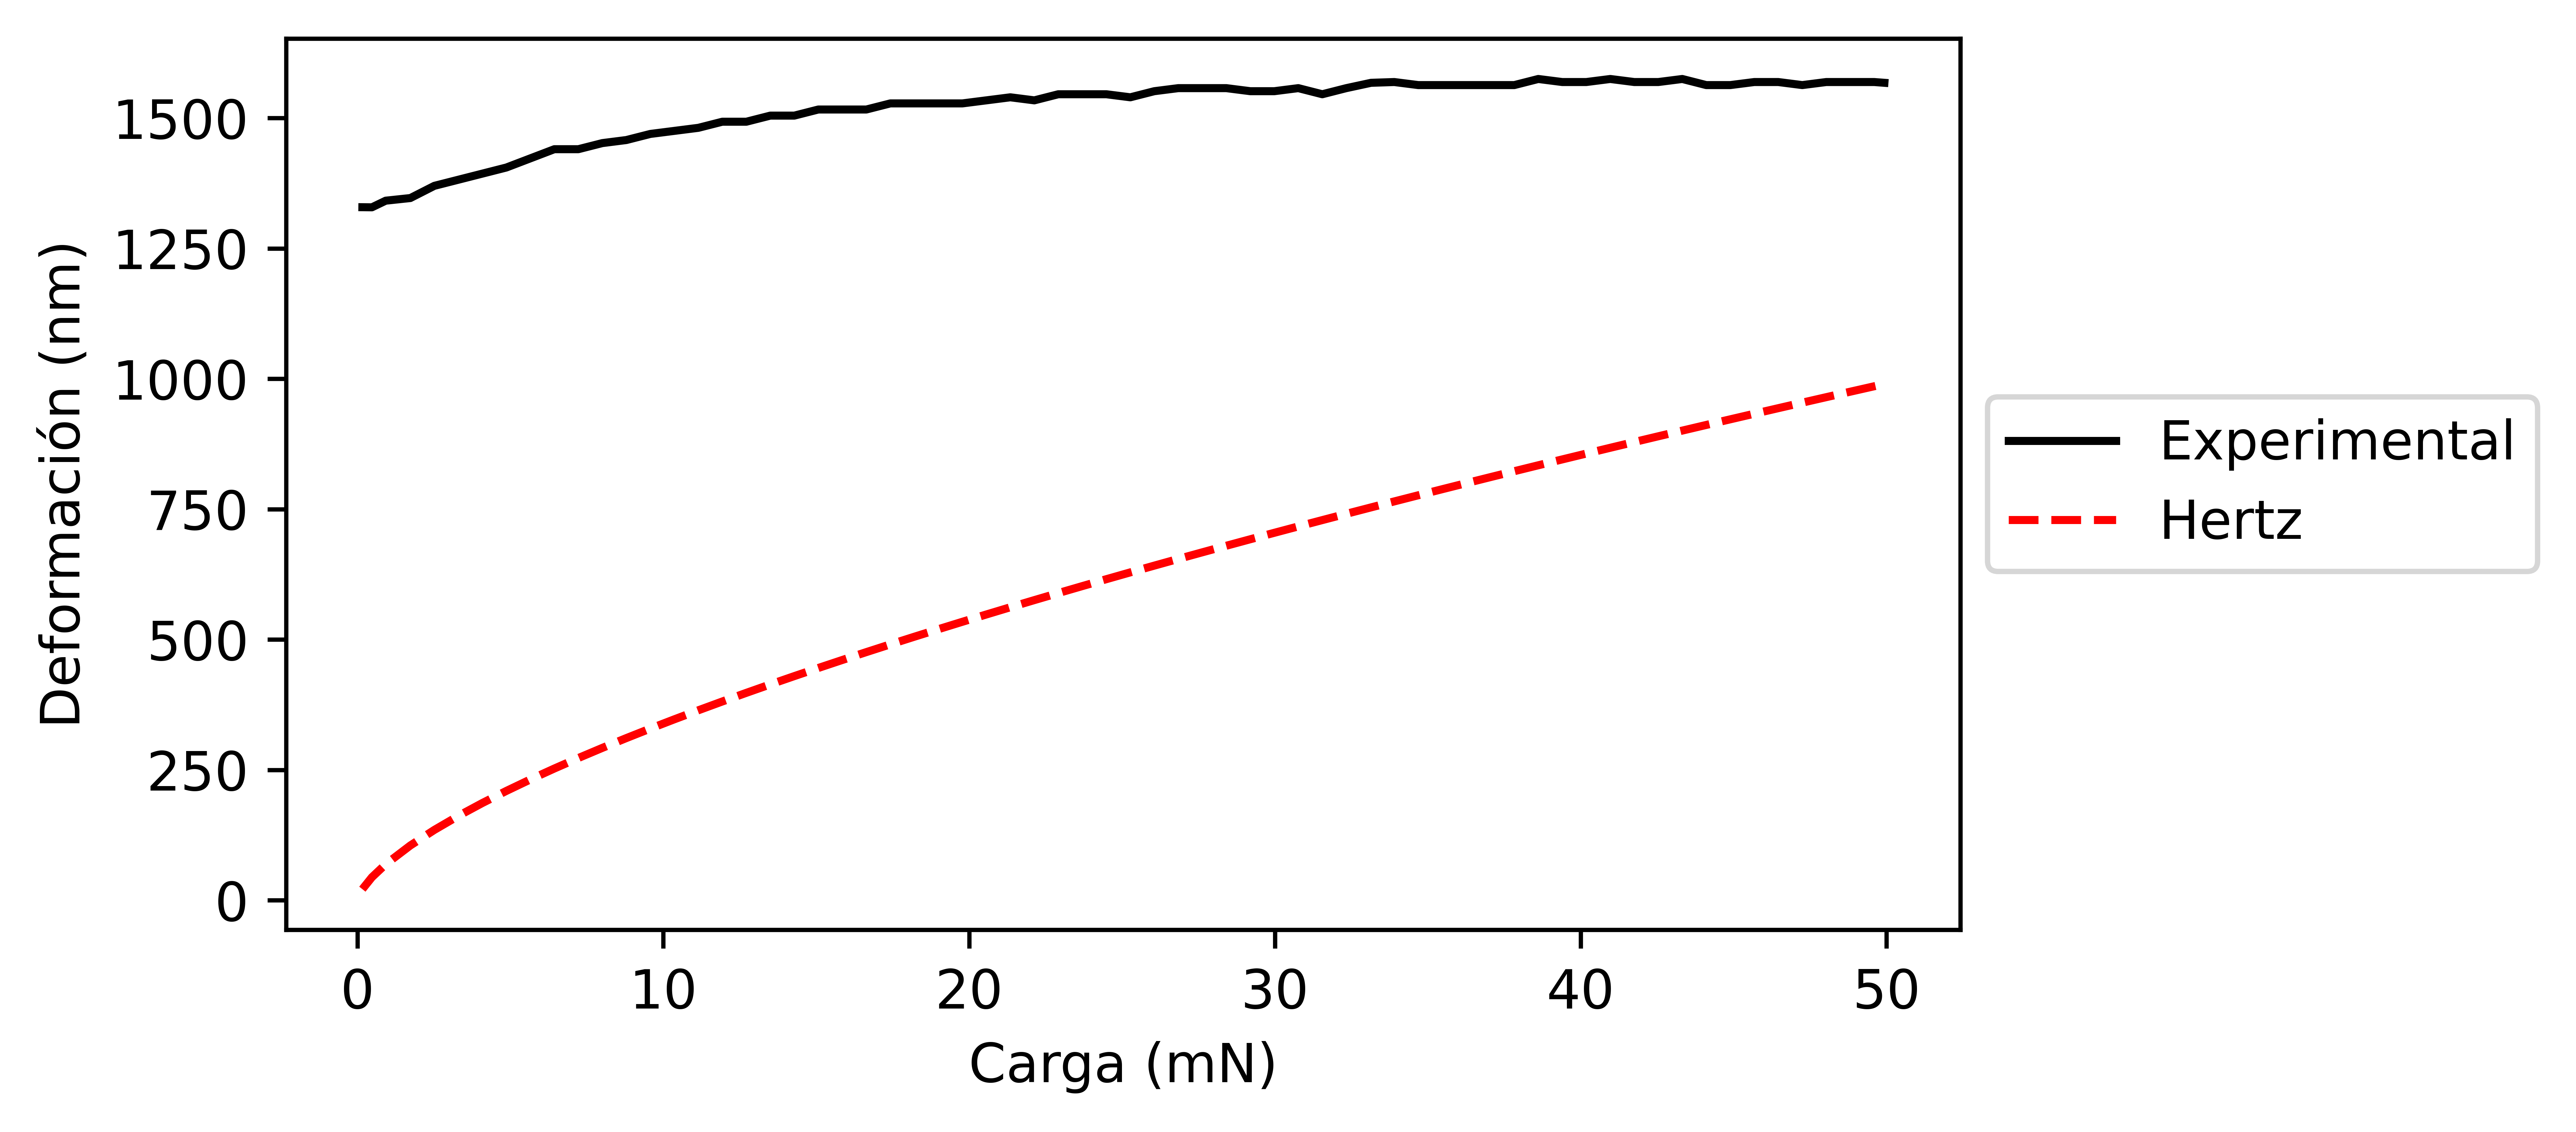
\includegraphics[width=\textwidth]{Images/pr_e_h.png}
         \caption{Gr\'aficas carga-profundidad de datos experimentales y modelo Hertziano.}
         \label{fig2a}
     \end{subfigure}
     \begin{subfigure}[t]{0.49\textwidth}
         \centering
         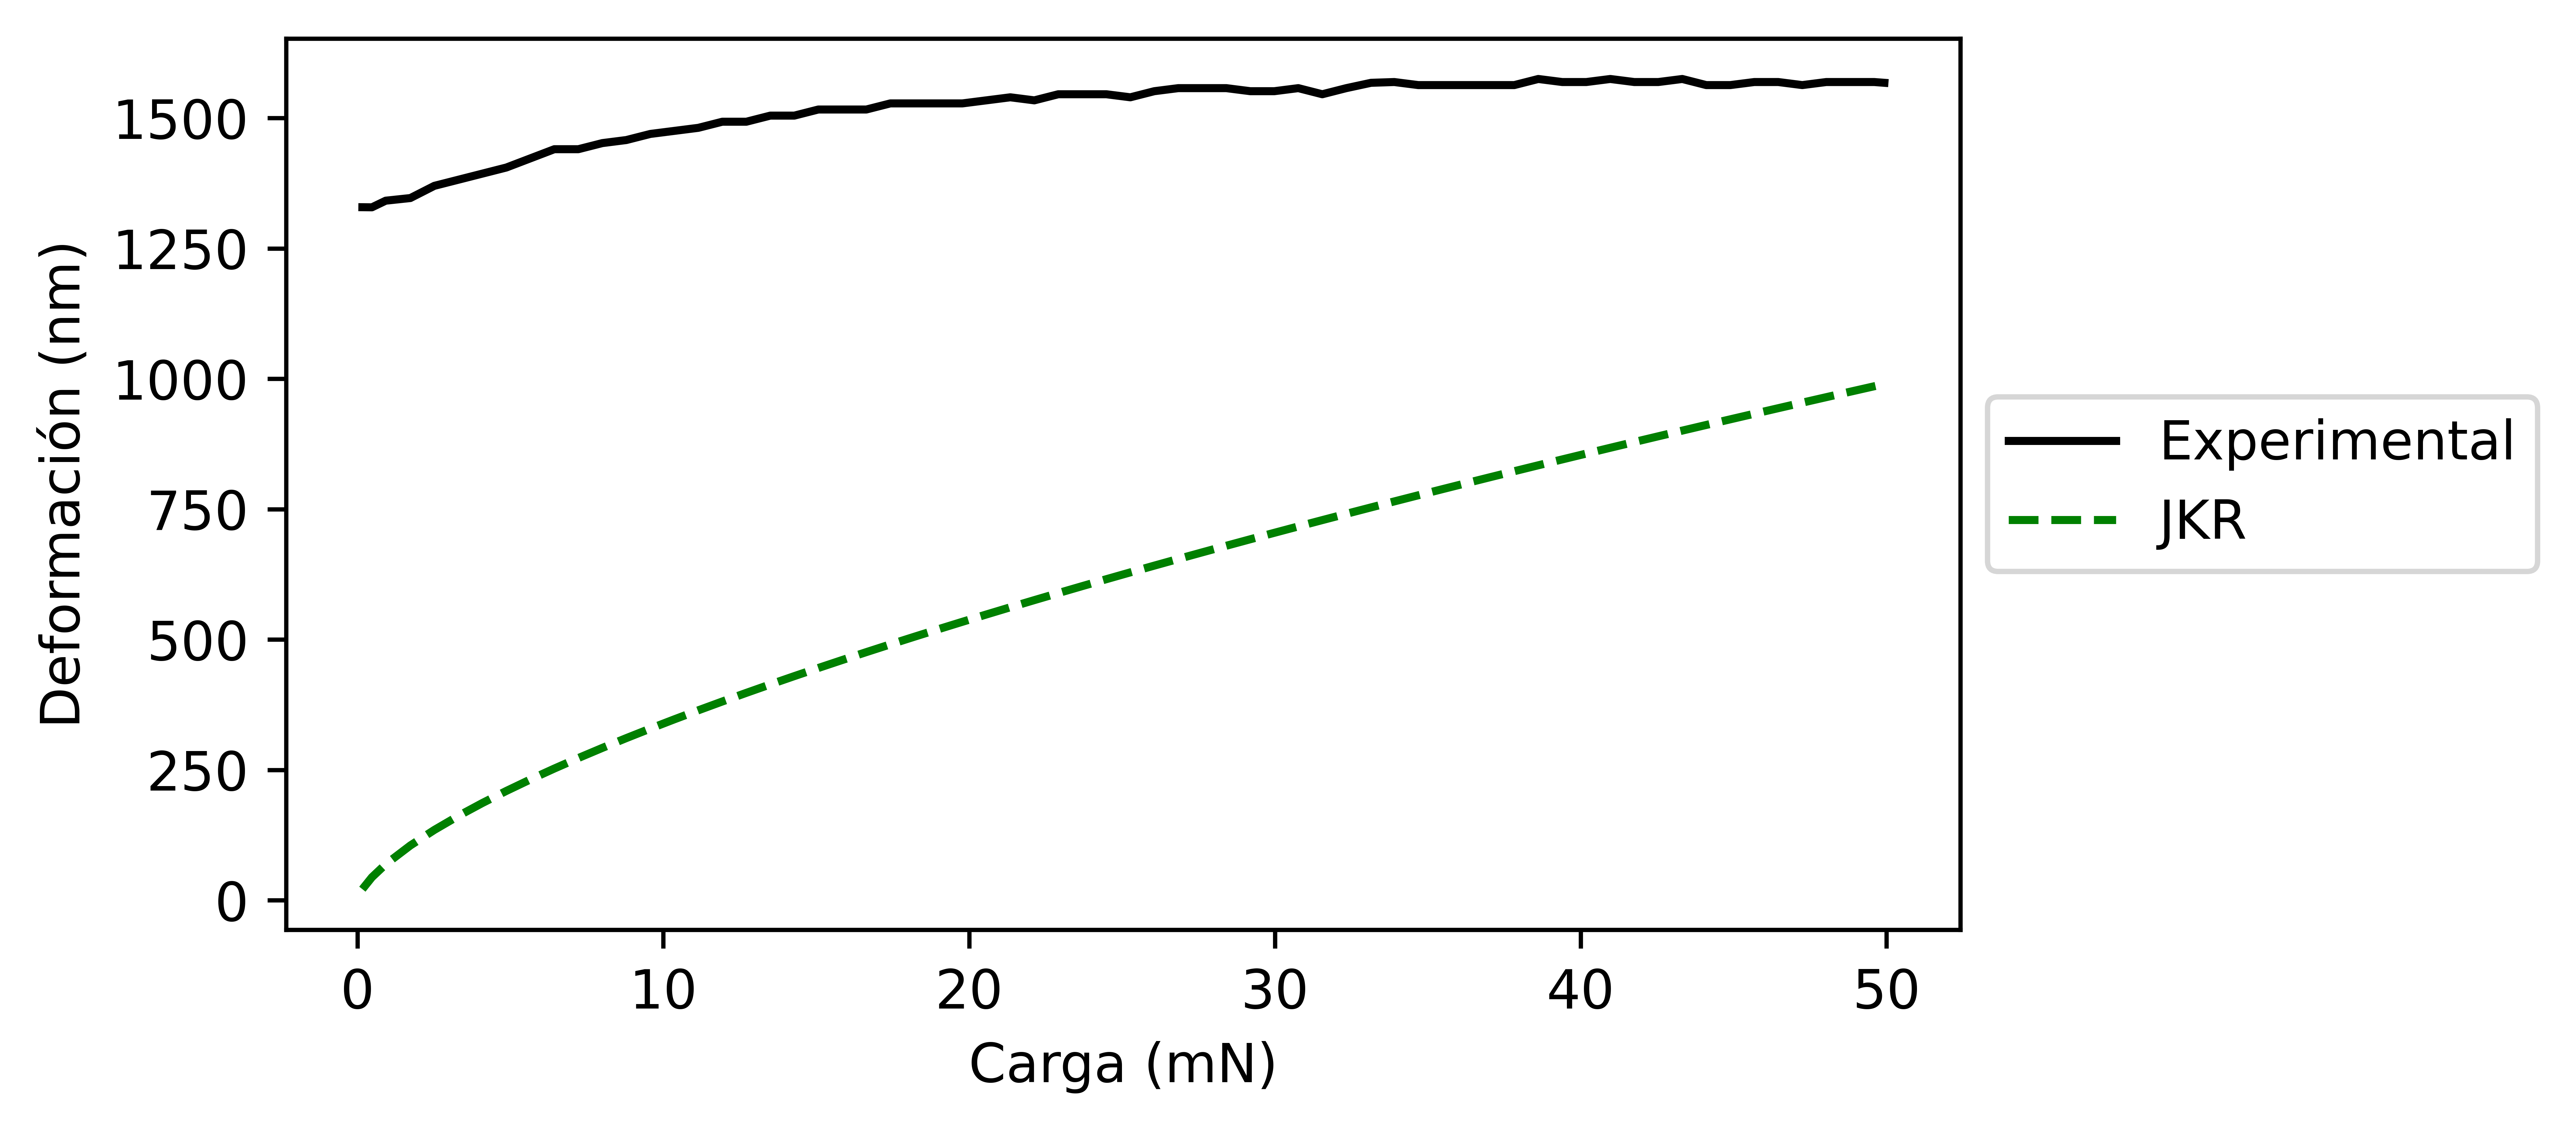
\includegraphics[width=\textwidth]{Images/pr_e_jkr.png}
         \caption{Gr\'aficas carga-profundidad de datos experimentales y modelo JKR.}
         \label{fig2b}
     \end{subfigure}
    \caption{Comparaciones entre datos experimentales y datos de los modelos Hertziano y JKR.}
    \label{fig2}
\end{figure}

\begin{figure}
\centering
    \begin{subfigure}[t]{0.49\textwidth}
         \centering
         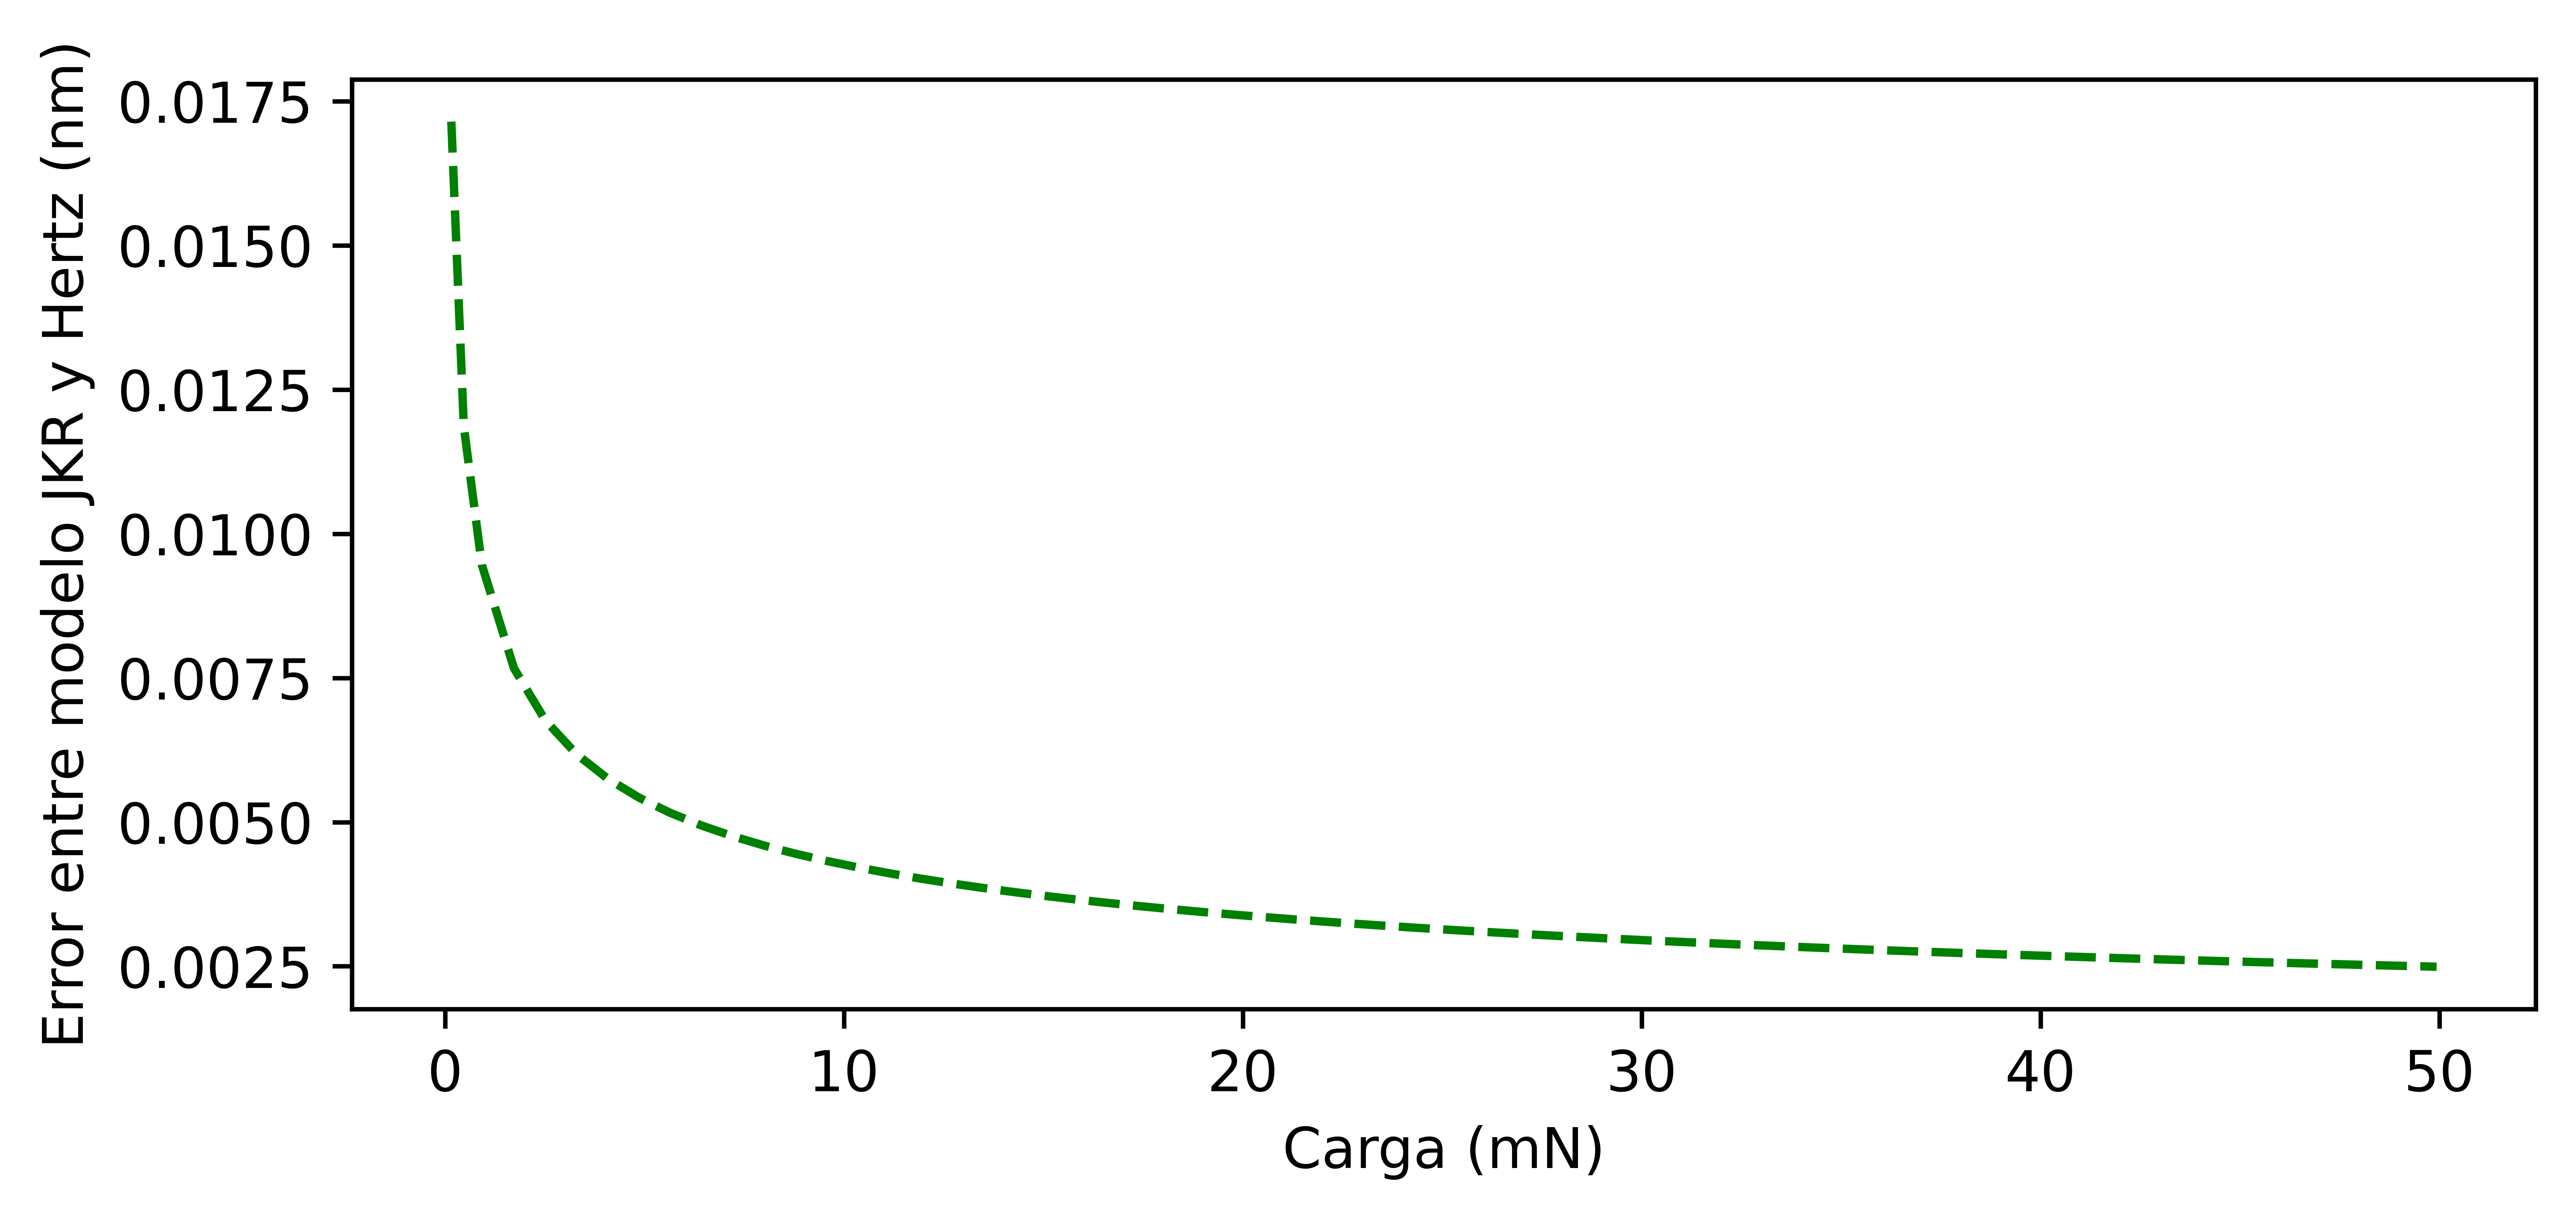
\includegraphics[width=\textwidth]{Images/diferencias_jkr_hertz.png}
         \caption{Error absoluto entre el modelo Hertziano y el JKR.}
         \label{fig3a}
     \end{subfigure}
     \begin{subfigure}[t]{0.49\textwidth}
         \centering
         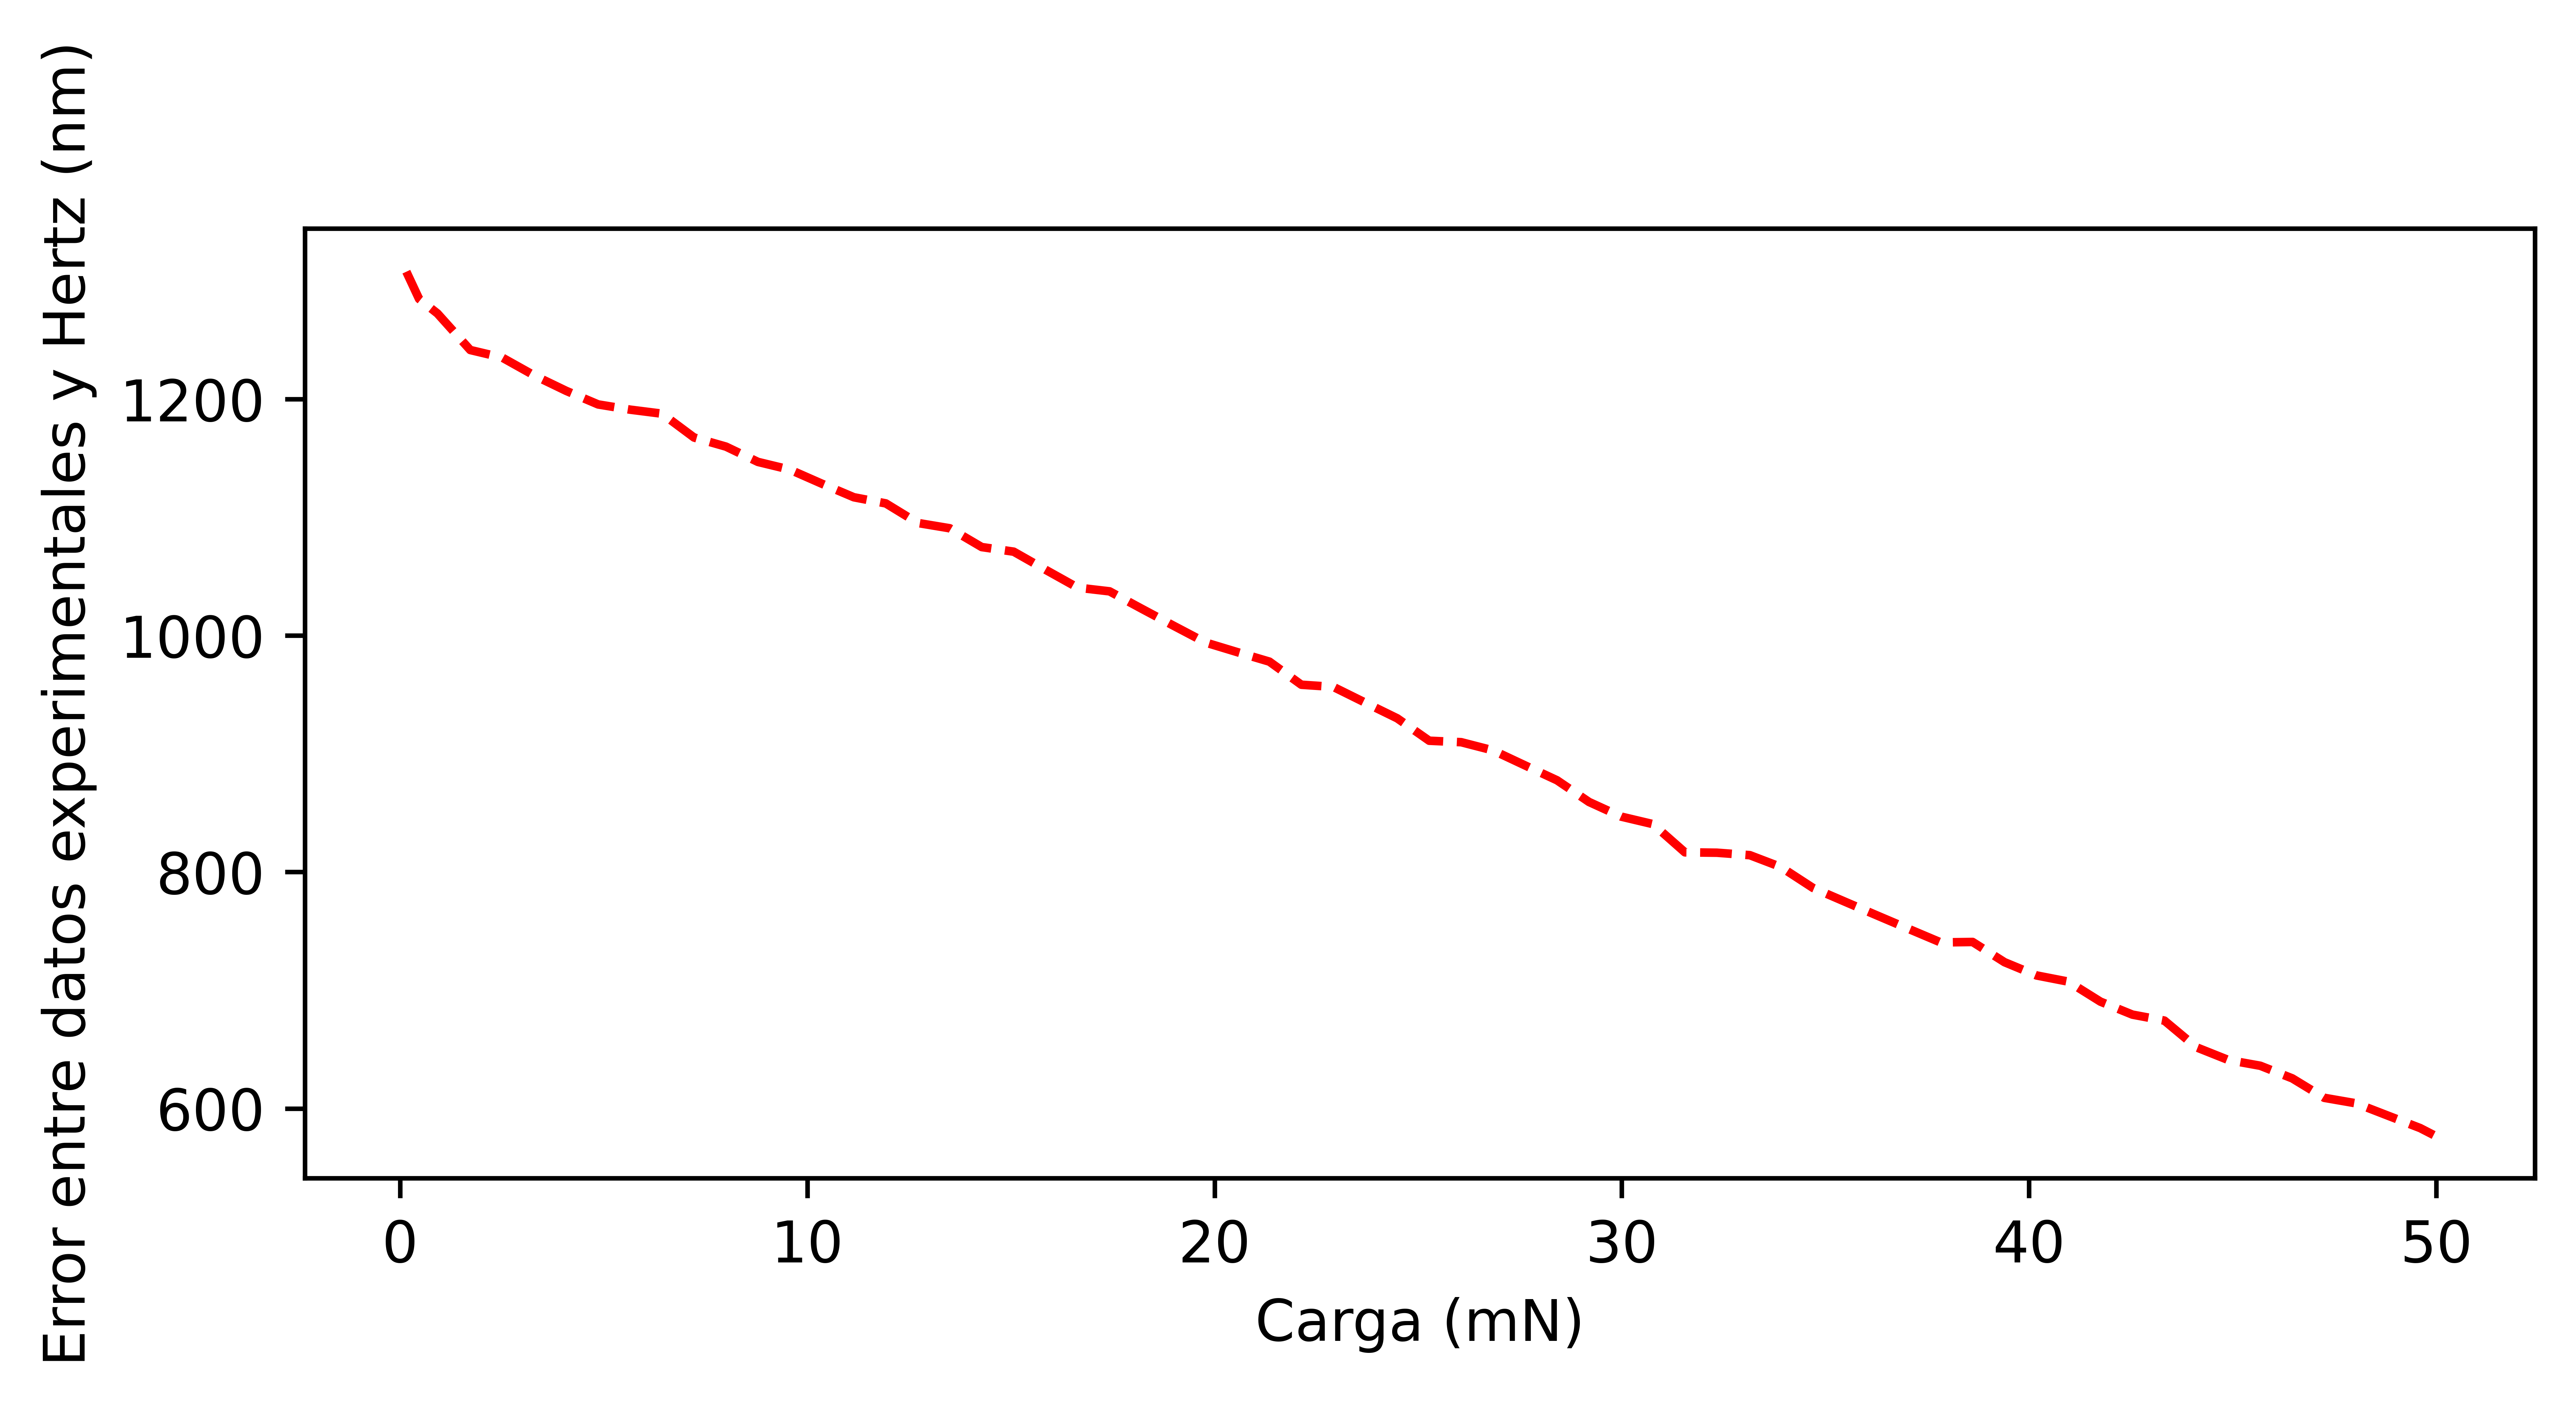
\includegraphics[width=\textwidth]{Images/diferencias_e_h.png}
         \caption{Error absoluto entre datos experimentales y el modelo Hertziano}
         \label{fig3b}
     \end{subfigure}
    \begin{subfigure}[t]{0.49\textwidth}
         \centering
         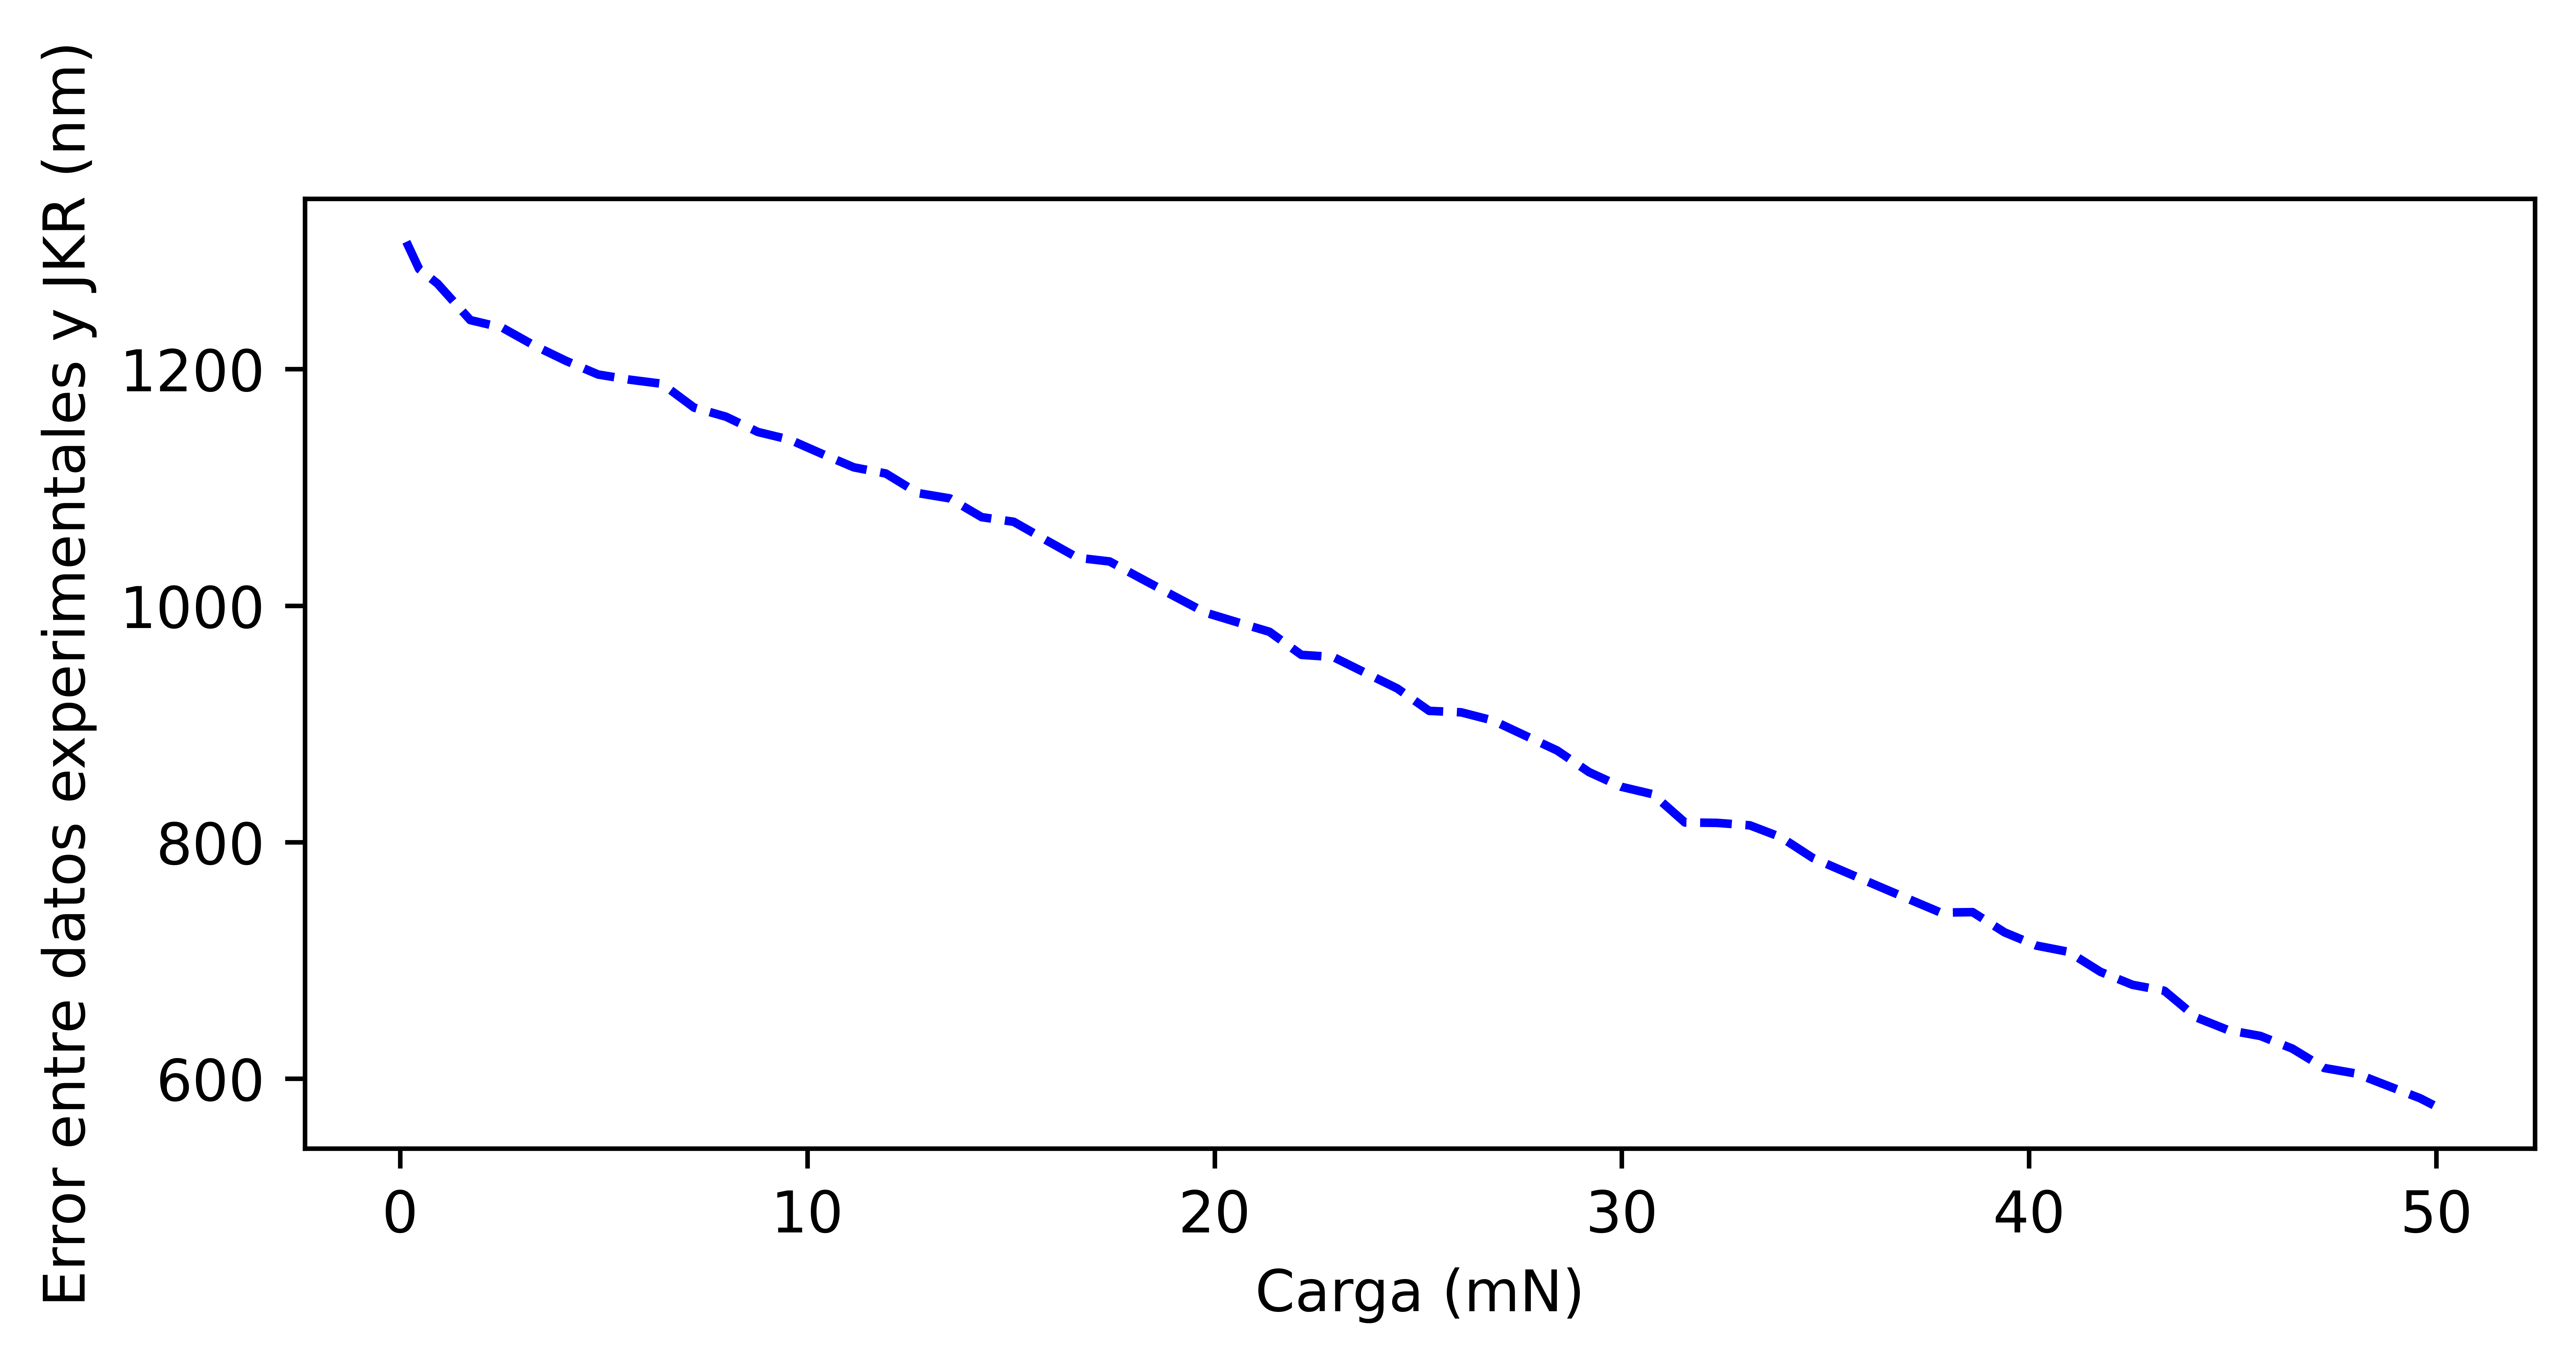
\includegraphics[width=\textwidth]{Images/diferencias_e_jkr.png}
         \caption{Error absoluto entre datos experimentales y el modelo JKR}
         \label{fig3c}
     \end{subfigure}
    \caption{Errores absolutos entre los datos experimentales y ambos modelos.}
    \label{fig3}
\end{figure}

\subsection{Discusi\'on}
Como se puede apreciar de la figura \ref{fig2}, no parece haber una gran diferencia entre las profundidades de indentaci\'on calculadas por ambos modelos, aunque s\'i que la hay al comparar con los datos experimentales. Sin embargo, parecen seguir una curvatura muy similar. Adem\'as, al comparar los errores absolutos entre el modelo Hertziano y el JKR, se puede percibir una gran diferencia a cargas bajas, mientras que esta disminuye a cargas mayores, justo como lo predicen dichos modelos. Lo mismo aplica al comparar cada uno de los modelos con los datos experimentales, excepto que en estas instancias las diferencias son mucho mayores.

\section{Conclusi\'on}
En el trabajo presente se opta por hacer una simulaci\'on muy directa, adem\'as de que no se toman en cuenta otros fen\'omenos como las fuerzas de fricci\'on existentes entre superficies, lo cual puede aumentar el \'area de contacto, aumentando a su vez la profundidad de indentaci\'on. Sin embargo, se comprueban las predicciones hechas por Johnson, Kendal y Roberts , en el que hay un aumento apreciable en cuanto a la profundidad de indentaci\'on a comparaci\'on con los estimados por Hertz, sobre todo a cargas aplicadas bajas, esto debido a las interacciones de adhesi\'on en las superficies.

\subsection{Trabajo a Futuro}
Debido al tiempo limitado del proyecto, no se ha podido realizar una simulaci\'on con un mayor grado de complejidad, en el que se implemente un modelo de din\'amica molecular y en el que se tomen en cuenta las interacciones entre \'atomos de la pel\'icula delgada de oro y la geometr\'ia del indentador de diamante. Adem\'as, se podr\'ian tomar en cuenta fuerzas de fricci\'on tangenciales, lo cual acercar\'ia los resultados de la simulaci\'on al comportamiento real de los materiales.

\bibliographystyle{elsarticle-num-names}
\bibliography{Referencias}

\end{document}
